\chapter{Related Works}
The EN–DE language pair has been examined in studies on gender bias, but research on dedicated bias detection systems is still limited. This chapter builds on the earlier definitions and reviews existing work to show how the problem has been addressed so far and where important gaps remain.

    \section{Literature Search Process}
        For the literature review, incremental and conceptual methods were combined, with each source leading to the identification of subsequent ones. Based on this progression, key concepts were identified and used to organize and interpret the literature, aligning with a conceptual approach. The structure followed the qualitative Information Systems framework by \textcite{schryenWritingQualitativeLiterature2015} and was further informed by \textcite{shresthaExploringGenderBiases2022} and \textcite{savoldiDecadeGenderBias2025}, both of whom conducted systematic reviews on gender bias in ML and MT respectively.

        Sources were primarily searched on \href{https://scholar.google.com/}{Google Scholar} and \href{https://www.perplexity.ai/}{Perplexity}, which served as an additional search engine. Prompts and outputs from Perplexity have been saved and are included in the appendix. To organize and manage the collected sources, \href{https://www.zotero.org/}{Zotero} was used throughout the process.

        \autoref{tab:key-concepts} defines the concepts that guided the literature search. Key search terms consisted of \textit{gender bias}, \textit{machine translation}, \textit{AI}, \textit{machine learning}, \textit{German}, \textit{stereotypes}, and \textit{detection}, which were combined with \textit{AND/OR}. The focus was on literature published between 2019 and 2025 to maintain relevance and currency, while foundational and definitional works from earlier periods were selectively included. The initial search for the term \textit{gender bias in machine translation} returned over 18,000 results. Through my iterative selection process, this was narrowed down to 34 core sources.

        \vspace{0.8em}
        \renewcommand{\arraystretch}{1.3}
            \begin{table}[ht!]
            \centering
            \begin{tabularx}{\textwidth}{>{\raggedright\arraybackslash}p{6.5cm}X}
            \toprule
            \textbf{Key Concept} & \textbf{Description} \\
            \midrule

            Defining Gender Bias in MT & Defines the core concept of gender bias in MT, including common bias patterns like gendered term insertion and incorrect gender assignments. Sets the conceptual foundation for the thesis. \\

            Relevance and Existing Research & Establishes the importance of studying gender bias by reviewing related work. Highlights key findings and their implications for fairness. \\

            Research Gaps and Open Challenges & Identifies the main gap: the absence of reliable detection systems for gender bias in EN-DE MT. Discusses the lack of a shared fairness definition and limitations in existing datasets. \\

            Technical Design and Implementation & Explains the theoretical background and fundamental principles necessary to understand the implementation. Covers the underlying concepts that guide design choices and system functionality. \\

            \bottomrule
            \end{tabularx}
            \caption{Key concepts relevant to this thesis}
            \label{tab:key-concepts}
        \end{table}

        Backward citation searching involved reviewing references cited by selected papers, prioritizing frequently cited and foundational works relevant to gender bias in MT. Forward citation searching used Google Scholar's "cited by" function to identify newer research citing those key papers. Filtering with specific terms (e.g., \textit{German} and \textit{machine translation}) was applied during forward search to maintain focus. Beyond these systematic methods, I also included supplementary sources when needed while writing. These consist of contextual references, statistics, or secondary citations that support specific points but were not part of the core conceptual or methodological framework. Supplementary sources were defined as materials identified outside the systematic search, such as papers found through backward citations or targeted queries for statistics and news, which provided support for subordinate arguments without being central to the study's theoretical or analytical structure. Titles and abstracts were manually screened to select relevant studies. Inclusion required sources to specifically address gender bias in MT, provide examples or discussions of gender-related errors, or explain the significance of gender bias in this context. Sources also had to be available in full text without access restrictions. Exclusion criteria filtered out studies focusing on general NLP bias without a direct link to MT, non-gender biases, and highly technical papers lacking contribution to the general understanding of gender bias or that did not provide additional knowledge beyond what was already found in previously published papers. Full texts were reviewed after initial screening to confirm relevance and extract insights. Redundant sources not providing new perspectives aligned with the thesis goals were excluded.
        
        \vspace{0.8em}
        \begin{table}[h]
            \centering
            \begin{tabularx}{\textwidth}{X X}
            \toprule
            \textbf{Inclusion Criteria} & \textbf{Exclusion Criteria} \\
            \midrule
            Addresses gender bias in MT & Focuses on general NLP bias without link to MT \\
            Provides examples or discussion of gender-related errors & Covers non-gender-related biases \\
            Explains the significance of gender bias in MT & Highly technical with no added general insight \\
            Available in full text without access restrictions & Redundant or not contributing new perspectives \\
            \bottomrule
            \end{tabularx}
            \caption{Selection criteria for literature review}
        \end{table}

    \section{Foundational studies}
        First mentions of this issue date back to over a decade ago, having been recognized by a paper by \textcite{schiebingerScientificResearchMust2014}. Since then, there has been a general increase in research papers focusing on this topic, especially between 2019 and 2023 \parencite{savoldiDecadeGenderBias2025}. \textcite{pratesAssessingGenderBias2019} conducted a large-scale study using Google Translate to translate sentences like "[Gender-neutral pronoun] is an engineer" from twelve gender-neutral languages into English. The results showed a strong bias toward male pronouns, especially in STEM occupations (see \autoref{fig:gt_surgeon_example} and \ref{fig:deepL_surgeon_example}). This could not be explained by real-world labour statistics, pointing instead to imbalances in the system's training data. The study received wide media attention, leading \citeauthor{googleReducingGenderBias2018} to change their translation policy: Google Translate began showing both feminine and masculine forms for ambiguous inputs \parencite{googleReducingGenderBias2018} (see \autoref{fig:gt_prates_example}).

        \vspace{0.8em}
        \begin{figure}[htb]
            \centering
            
\includegraphics[width=1\textwidth]{gt_surgeon_example.png}
            \caption[Example of Google Translate's biased translation]{Google Translate translates an occupational term with a gender stereotype, using the masculine form for "surgeon"}
            \label{fig:gt_surgeon_example}
        \end{figure}

        \vspace{0.8em}
        \begin{figure}[htb]
            \centering
            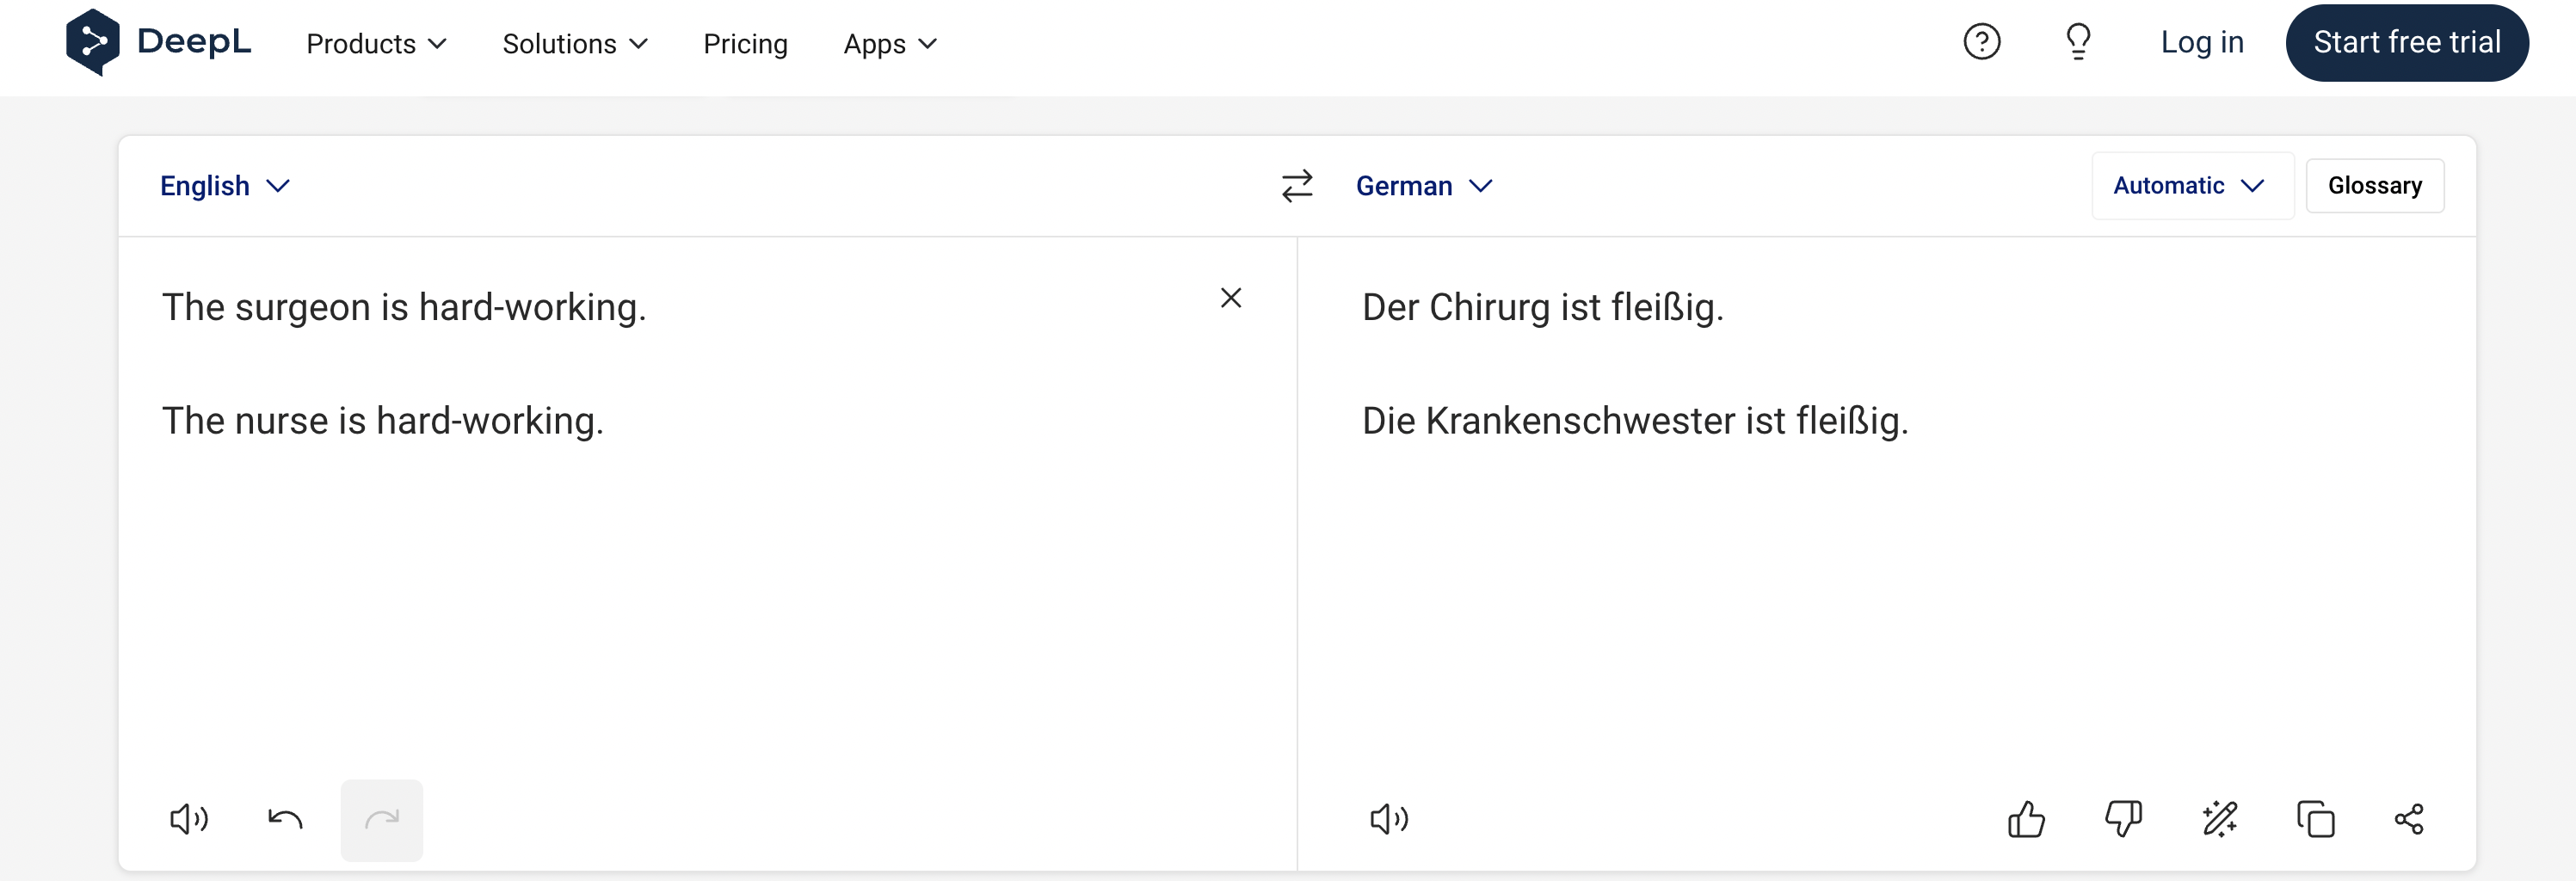
\includegraphics[width=1\textwidth]{deepL_surgeon_example.png}
            \caption[Example of DeepL's biased translation]{DeepL translates the same occupational term with a gender bias, mirroring Google Translate's masculine default for "surgeon"}
            \label{fig:deepL_surgeon_example}
        \end{figure}

        \vspace{0.8em}
        \begin{figure}[htb]
            \centering
            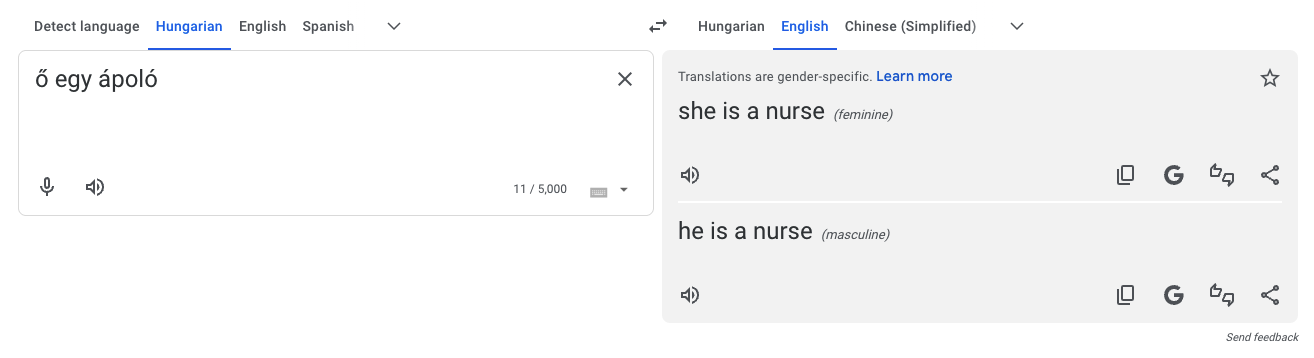
\includegraphics[width=1\textwidth]{gt_prates_example.png}
            \caption[Google Translate Gendered Pronoun Suggestions]{Google Translate assigns gendered pronouns in translation for an originally gender-ambiguous subject}
            \label{fig:gt_prates_example}
        \end{figure}

        Building on this, \textcite{stanovskyEvaluatingGenderBias2019} created WinoMT, a benchmark for evaluating gender bias in English-to-multilingual translations. It focused on occupations in contexts designed to challenge stereotypes. The study found that systems were more accurate for stereotypical gender roles but struggled in non-stereotypical cases, confirming the trends observed by \citeauthor{pratesAssessingGenderBias2019}.
        Together, these studies helped spark the ongoing research interest in gender bias in MT.

        According to \textcite{ullmannGenderBiasMachine2022}, translation errors stem from biases present in the training data. The MT systems learns gender associations from word co-occurrences, such as “doctor” with masculine pronouns, causing incorrect or inserted gender in translations. It also amplifies existing biases during training like linking cooking predominantly with women, which leads to gendered outputs not supported by the input. The large size of training corpora increases the challenge of controlling data quality. Manual inspection becomes impractical when models are trained on hundreds of billions of tokens. Consequently, the model can unintentionally absorb and reproduce harmful or biased content, reinforcing patterns that lead to biased translations \citep{ullmannGenderBiasMachine2022}.

    \section{Implications of Bias}
        Biases do not only cause translation errors but also have wider social consequences. They can lead to representational harm by repeatedly portraying certain genders in limiting or stereotypical ways \parencite{stanczakSurveyGenderBias2021}. Since these biased outputs can re-enter the training data and influence future MT models, the cycle of biased representation continues and reinforces itself in society, creating a regressive feedback loop. The generic masculine in particular leads to inaccurate and unfair representations of gender in translated text. \textcite{rescignoGenderBiasMachine2023} observed a predominance of masculine forms in translation outputs (approximately 90\% in Google Translate and 85–88\% in DeepL for EN-IT and EN-DE), even when the original sentences contained relatively few masculine references. This shows that the bias is not minor but occurs quite heavily in those systems. It also contributes to the invisibility of women in male-dominated professions \parencite{kapplAreAllSpanish2025}. Studies show that biased language in machine-generated text, such as children’s stories or job ads, can influence how young people view themselves \parencite{soundararajanInvestigatingGenderBias2024,kapplAreAllSpanish2025}. It may shape their interests, hobbies, and career choices. This is especially visible in STEM fields \parencite{pratesAssessingGenderBias2019}, where stereotypes are more persistent. When job descriptions or mock interviews use gender-exclusive pronouns, women report feeling less belonging, lower motivation, and weaker identification with the role \parencite{godsilEffectsGenderRoles2016}. Many self-select out of applying, shrinking the female talent pool and reinforcing gender gaps in the workforce.


        \vspace{0.8em} 
        \begin{figure}[htb]
            \centering
            \scalebox{0.8}{
\begin{tikzpicture}[
    box/.style={rectangle, draw, rounded corners, minimum width=2.5cm, minimum height=1.2cm, align=center, font=\small},
    arrow/.style={-Stealth, thick, shorten >=1pt, shorten <=1pt},
    label/.style={midway, font=\footnotesize\bfseries}
]

\node[box] (bias) {Gender Bias\\in Society};
\node[box, right=3.5cm of bias] (data) {Training Data};
\node[box, right=3.5cm of data] (mt) {MT System};
\node[box, below=2.5cm of mt] (output) {Biased\\Outputs};
\node[box, below=2.5cm of bias] (harm) {Representational\\Harm};

\draw[arrow] (bias) -- (data) node[label, above] {1. Reflects};
\draw[arrow] (data) -- (mt) node[label, above] {2. Trains};
\draw[arrow] (mt) -- (output) node[label, right=3mm, xshift=2mm] {3. Produces};  
\draw[arrow] (output) -- (harm) node[label, above] {4. Causes};
\draw[arrow] (harm) -- (bias) node[label, left=3mm, xshift=-2mm, yshift=1mm] {5. Reinforces}; 

\end{tikzpicture}
}
            \caption{Regressive feedback loop of gender bias in MT}
            \label{fig:regressive_feedback_loop}
        \end{figure}
        \vspace{0.8em} 


        Research also shows that using Gender-Fair Language (GFL) like "she and he" or "one" can improve how women respond to job ads. It reduces stereotype threat and helps them engage more positively with opportunities \parencite{godsilEffectsGenderRoles2016}. Furthermore, a study by \textcite{savoldiWhatHarmQuantifying2024} measured how much effort people need to fix biased translations. They used metrics like the time it took to edit and how many edits were needed, based on human-targeted error rate. The results showed that fixing translations with feminine forms took almost twice as long and required four times more edits than those with masculine forms. As a result, biased translations lead to higher economic costs and a quality gap that disproportionately affects women. \textcite{savoldiWhatHarmQuantifying2024} argued that current automatic bias metrics miss these human impacts. They called for better evaluation methods that reflect what users actually experience.

    \section{English-German Linguistic Challenges}
        Although both English and German originate from the Indo-European language family \parencite{baldiEnglishIndoEuropeanLanguage2008}, they have different liguistic characteristcs. English does not assign grammatical gender to nouns. The article "the" is used universally, independent of what it refers to. On the contrary, German assigns one of three grammatical gendered articles to nouns: "der" (m), "die" (f) and "das" (n). The form or ending of a noun may also change depending on its grammatical gender. While English has a few gendered word pairs, such as "actor" (m) and "actress" (f), gender distinctions in German apply broadly across the entire noun system. "Der Student" refers to a male student, whereas "die Studentin" refers to a female student. 

        Note that grammatical gender has no connection to societal or biological gender. It is a rule of the language rather than a reflection of identity. For example, the German word Mädchen (girl) is grammatically neuter and takes the article "das". This is not because the referent lacks gender, but because the suffix "-chen" automatically assigns neuter gender. Grammatical gender in German follows structural rules, even when they contradict real-world gender associations.

    \subsubsection{German Gender-Fair Language} \label{subsection:german_gfl}
    GFL is the use of language that treats all genders equally and aims to reduce stereotyping and discrimination \parencite{sczesnyCanGenderFairLanguage2016}. Three common approaches to plural mentionings in German are: 

    \begin{itemize}
        \item \textbf{Gender-neutral rewording:}  
        This uses neutral terms instead of gendered nouns, e.g., \textit{die Studierenden lernen}. A challenge for this version is that neutral alternatives do not exist for every noun and cannot be consistently applied \parencite{lardelliBuildingBridgesDataset2024}.

        \item \textbf{Gender-inclusive characters:}  
        This combines masculine, feminine and non-binary forms by using a character like \textit{*}, \textit{:}, or \textit{\_}, e.g., \textit{die Student*innen lernen}. This method is consistent but may interrupt reading flow and lacks standardization \parencite{lardelliBuildingBridgesDataset2024}.

        \item \textbf{Pair form:}  
        This names both gender forms, e.g., \textit{die Studentinnen und Studenten lernen}. It is currently the most used GFL form in German \parencite{waldendorfWordsChangeIncrease2024}, briefly surpassing the star and colon characters as seen in \autoref{fig:gfl_types_frequency}.
    \end{itemize}

    \vspace{0.8em}
    \begin{figure}[htb]
        \centering
            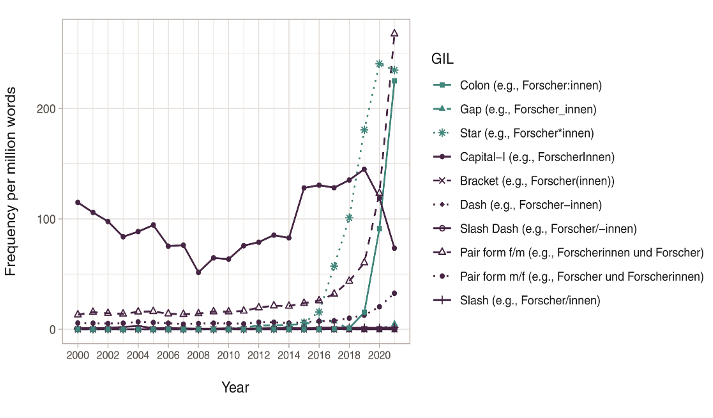
\includegraphics[width=1\textwidth]{gfl_types_frequency.png}
        \caption[Frequency of different types of gender-inclusive language]{Frequency of different types of gender-inclusive language. Source: \textcite{waldendorfWordsChangeIncrease2024} p. 367}
        \label{fig:gfl_types_frequency}
    \end{figure}

    These examples apply when the gender of the subjects is ambiguous. But when gender is known, especially in singular mentions, the generic masculine should be avoided. However, in the same way as gender bias has no clear definition, there is no agreed standard for GFL \parencite{lardelliBuildingBridgesDataset2024, savoldiDecadeGenderBias2025}. "Fairness" therefore heavily depends on personal views, culture, and context, which raises ethical questions about debiasing systems. 
    The use of GFL has increased in recent years \parencite{waldendorfWordsChangeIncrease2024}, but it remains generally low. This results in a scarcity of relevant linguistic data. Few datasets include GFL variants, and existing resources often rely on manual translations or post-editing to add gender-inclusive forms \parencite{lardelliBuildingBridgesDataset2024}. 

    % --------------------------------------------------------------------------------

    \section{Research Gaps}
    A central gap in gender bias research is the absence of a shared definition of what constitutes "fair" language. This lack of conceptual clarity makes it difficult to design systematic evaluation approaches, define accountability standards, or detect all relevant forms of harm \parencite{barclayInvestigatingMarkersDrivers2024a,shresthaExploringGenderBiases2022,stanczakSurveyGenderBias2021}. A second major gap concerns the availability of high-quality EN-DE translation data containing GFL. While a few datasets exist, they are not designed for bias detection and often require manual post-editing to include inclusive forms \parencite{lardelliBuildingBridgesDataset2024}. This lack of consistent GFL examples limits the ability to develop and evaluate models in a structured and reproducible way, and makes it harder to train systems to recognize gender-fair alternatives as neutral.

    \textcite{stanczakSurveyGenderBias2021} note that findings on gender bias in English do not always apply to other languages such as German. Linguistic differences make language-specific approaches necessary. Studies on EN–DE systems \parencite{ullmannGenderBiasMachine2022,kapplAreAllSpanish2025,lardelliBuildingBridgesDataset2024} confirm the presence of gender bias, propose mitigation strategies, or introduce evaluation metrics. Yet, only a few focus on systematic methods to detect bias in translated text. This study addresses that gap by treating bias detection as a prerequisite for any effective mitigation strategy. Since reliable automatic debiasing techniques are not yet available, manual intervention will remain necessary in practice. The primary objective is therefore to identify biased translations with high accuracy, providing a basis for subsequent correction or debiasing efforts.

% --------------------------------------------------------------------------------

